\documentclass[12pt]{article}

\usepackage[utf8]{inputenc}
\usepackage{amsmath}
\usepackage{amsfonts}
\usepackage{amssymb}
\usepackage{graphicx}
\usepackage{url}
\usepackage{xcolor}
\definecolor{linkcolor}{RGB}{77,77,77} % black!70 equivalent
\usepackage[colorlinks=true,
            allcolors=linkcolor,
            linkcolor=linkcolor,
            citecolor=linkcolor,
            urlcolor=linkcolor,
            breaklinks=true]{hyperref}
\usepackage{nameref}
\usepackage{tikz}
\usetikzlibrary{positioning,decorations.markings,decorations.pathmorphing}
\usepackage{helvet}
\usepackage{titlesec}
\usepackage{geometry}
\usepackage{multicol}
\usepackage{soul} % For underline effects
\usepackage{fancyhdr} % For fancy headers
\usepackage{float} % For precise figure placement

% Set modern margins
\geometry{
    top=2.00cm, % 1 inch from top
    bottom=2.5cm,
    left=2.5cm,
    right=2.5cm,
    headsep=0.75cm % Quarter inch of space between header and text
}

% Add space above header
\setlength{\headheight}{24pt}
\addtolength{\topmargin}{1cm}

% Define colors
\definecolor{darkgray}{RGB}{50,50,50}

% Epic styling for sections
\titleformat{\section}
    {\Huge\bfseries\centering}
    {}
    {0em}
    {\MakeUppercase}
    [{\centering
    \begin{tikzpicture}
    \draw[line width=1.5pt] (-0.4\textwidth,0) -- (-0.1,0);
    \draw[line width=1.5pt] (0.1,0) -- (0.4\textwidth,0);
    \draw[fill=darkgray] (-0.1,-0.15) -- (0,0.15) -- (0.1,-0.15) -- cycle;
    \end{tikzpicture}
    \vspace{1em}}]

\titleformat{\subsection}
    {\Large\bfseries}
    {\thesubsection.}
    {1em}
    {\MakeUppercase}


% Epic header/footer style
\pagestyle{fancy}
\fancyhf{}
\renewcommand{\headrulewidth}{0pt}
\fancyhead[L]{\small\MakeUppercase{\textbf{RandAO}}}
\fancyhead[R]{\small\textbf{\thepage}}
\fancyhead[C]{\vspace{0.5em}\rule{\textwidth}{0.5pt}}

% Custom page style for first pages of chapters
\fancypagestyle{plain}{%
    \fancyhf{}
    \renewcommand{\headrulewidth}{0pt}
    \fancyfoot[C]{%
        \vspace{-1cm}
        \rule{0.3\textwidth}{0.5pt}
        {\small\thepage}
        \rule{0.3\textwidth}{0.5pt}
    }
}

% Redefine section title spacing
\titlespacing*{\section}{0pt}{1.5em}{0.5em} % Space after reduced to 0.5em
\titlespacing*{\subsection}{0pt}{2em}{1em} % Kept the same

% Set default font to Helvetica
\renewcommand{\familydefault}{\sfdefault}

% Custom spacing
\setlength{\parskip}{1em}
\setlength{\parindent}{0pt}

% Example environment
\newtheorem{example}{Example}

% Load title page definition
% Define hexagon shape
\newcommand{\hexagon}[1]{
    \draw[black!10, line width=0.3pt] 
    (0,0) -- (60:#1) -- (120:#1) -- (180:#1)
    -- (240:#1) -- (300:#1) -- cycle;
}

% Custom title page
\makeatletter
\def\maketitle{
    \begin{titlepage}
        \begin{tikzpicture}[overlay, remember picture]
            % Hexagonal background pattern
            \foreach \i in {-400,-360,...,400} {
                \foreach \j in {-600,-520,...,600} {
                    \begin{scope}[shift={([xshift=\i pt,yshift=\j pt]current page.center)}]
                        \hexagon{40pt}
                    \end{scope}
                }
            }
            \foreach \i in {-380,-340,...,380} {
                \foreach \j in {-560,-480,...,560} {
                    \begin{scope}[shift={([xshift=\i pt,yshift=\j pt]current page.center)}]
                        \hexagon{40pt}
                    \end{scope}
                }
            }
            
            % Center point for vertical alignment
            \path (current page.center) ++(0,6cm) coordinate (title center);
            
            % Title and tagline group
            \begin{scope}[local bounding box=title-group]
                % Title
                \node[inner sep=2pt, align=center, anchor=center] at (title center) (title) {
                    \scalebox{4.5}{
                        \textcolor{black}{\textbf{\textsf{RandAO}}}
                    }
                };
                
                % Decorative elements around title
                \draw[line width=0.5pt] ([xshift=-3cm]title.west) -- ([xshift=-0.5cm]title.west);
                \draw[line width=0.5pt] ([xshift=0.5cm]title.east) -- ([xshift=3cm]title.east);
                
                % Tagline
                \node[below=0.8cm of title, font=\Large, align=center] (tagline) {
                    \textcolor{black!70}{\textsf{Version 2 \textbar{} Any-Honest Time-Lock Randomness for AO \textbar{} \$RNG}}
                };
                
                % Horizontal line under tagline
                \draw[line width=1pt] 
                    ([yshift=-0.75cm]tagline.south west) -- 
                    ([yshift=-0.75cm]tagline.south east);
            \end{scope}
            
            % Favicon image centered and positioned relative to page center
            \path (current page.center) ++(0,-2cm) coordinate (favicon-pos);
            \node[inner sep=0pt] at (favicon-pos) {
                
\includegraphics[width=5cm]{images/favicon.png}
            };
            
            % Date at bottom
            \node[align=center] at ([yshift=2cm]current page.south) {\large\textsf{\@date}};
            
            % Corner decorations
            \foreach \corner in {north east, north west, south east, south west} {
                \draw[line width=0.5pt] 
                    ([xshift=-1cm, yshift=-1cm]current page.\corner) -- 
                    ([xshift=1cm, yshift=1cm]current page.\corner);
            }
        \end{tikzpicture}
    \end{titlepage}
}
\makeatother


\title{RandAO v2}
\author{}
\date{\today}

\begin{document}

\pagenumbering{roman}
\maketitle

{\centering
\Huge\bfseries\MakeUppercase{Contributors}

\vspace{0.3em}
\begin{tikzpicture}
\draw[line width=1.5pt] (-0.4\textwidth,0) -- (-0.1,0);
\draw[line width=1.5pt] (0.1,0) -- (0.4\textwidth,0);
\draw[fill=darkgray] (-0.1,-0.15) -- (0,0.15) -- (0.1,-0.15) -- cycle;
\end{tikzpicture}
\par}
\vspace{1em}

\begin{center}
\makebox[\textwidth]{%
\begin{tabular}{@{\hspace{2em}}c@{\hspace{2em}}c@{\hspace{2em}}c@{\hspace{2em}}}
    {\LARGE\textbf{Allan B. Pedin IV}} &
    {\LARGE\textbf{Alex Posey}} &
    {\LARGE\textbf{Tyler Warburton}} \\[0.2em]
    {\color{gray}\textsc{Kenny Swayzee}} &
    {\color{gray}\textsc{Caitlyn Lane}} &
    {\color{gray}\textsc{Ethan Gold}}
\end{tabular}%
}
\end{center}

\clearpage

\section*{Abstract}
RandAO is a suite of cryptographic tools for the new age of the internet, built on HyperBEAM. It starts with randomness. HyperBEAM v0.11-RC7 sandboxes \texttt{math.random}, because a value drawn from a node's own generator differs between nodes and replays and can be steered by whoever picks the seed. RandAO brings it back safely: one Lua library gives every AO process deterministic randomness for free, and upgrades the same call to verifiable randomness when value is at stake. Its flagship tier is an any-honest commit-reveal of time-lock puzzles: every validator commits a puzzle whose answer is fixed when posted but cannot be computed by anyone else before the commitment window closes, then reveals it with the puzzle's one-time trapdoor. The node checks each reveal with a single modular exponentiation through the \texttt{timelock@1.0} device; a validator that withholds is cracked by the others, who prove their work with a Wesolowski proof. As long as one validator is honest, nobody can predict or bias a draw. A fast threshold-signature tier and a free local tier sit beside it, and time-lock encryption is next, all from the same library and device. Requests are paid in the \$RNG token: one token to each validator that served a request and one to the protocol.

\clearpage
\tableofcontents

\clearpage
\pagenumbering{arabic}
\section{Introduction}\label{sec:introduction}


\subsection{Motivation}\label{sec:motivation}

Random values have been a fundamental building block of Web2 applications, powering everything from gaming mechanics to cryptographic protocols. As we transition to Web3, we must maintain these essential capabilities while upholding our core principles of decentralization and security. However, blockchain's inherently deterministic and public nature presents a unique challenge in preserving the unpredictability of random values.

This fundamental limitation creates what we term the ``\textbf{Onchain Randomness Problem}'': as soon as entropy becomes available on the blockchain, all outcomes dependent on that entropy become predictable by any observer. Traditional attempts to generate randomness within blockchain systems have led to various compromises in security, integrity, or decentralization, undermining the very principles Web3 aims to uphold.

\subsection{Bringing Back \texttt{math.random}}\label{sec:math_random}

On AO the problem is now concrete. Release v0.11-RC7 of HyperBEAM, the node software that runs AO processes, replaces \texttt{math.random} in its Lua runtime with a sandboxed placeholder, together with \texttt{os.time}, \texttt{os.clock} and \texttt{os.date}. Each of these returns a value that depends on the node running it: its random seed, its clock, its time zone. That makes them unsafe in two ways:

\begin{itemize}
    \item \textbf{Forks}: an AO process is defined by replaying its messages. If two nodes, or the same node on a replay, draw different numbers, they compute different states for the same process, and its history forks.
    \item \textbf{Manipulation}: whoever controls the seed controls the draw. A node operator can choose or observe the seed and predict or steer every roll, which makes node-local randomness worthless for anything of value.
\end{itemize}

RandAO brings \texttt{math.random} back safely. A single call, \texttt{rng.install(msg)}, gives \texttt{math.random} a deterministic stream derived from the message, identical on every node and every replay, so existing code keeps working at no cost. When a draw carries value, \texttt{rng.request} upgrades the same code to verifiable randomness from the network, at the security level the application chooses.

\subsection{Our Contribution}\label{sec:our_contribution}

RandAO is a suite of cryptographic tools for the new age of the internet, delivered through one library and one HyperBEAM device. Its first tool is tiered randomness; time-lock encryption follows. The flagship is the second version of the time-lock protocol RandAO was founded on, rebuilt for HyperBEAM:

\begin{itemize}
    \item \textbf{Any-Honest Security}: The output is unpredictable and unbiasable as long as at least one committed validator is honest.

    \item \textbf{Withholding Cannot Bias}: Once commitments close, every contribution is fixed. A validator that refuses to reveal is cracked; the worst it can do is delay the round.

    \item \textbf{Verification on the Node}: A reveal carries the puzzle's one-time trapdoor, so the node checks it with one modular exponentiation through the \texttt{timelock@1.0} device. Cracks carry a Wesolowski proof. No verifier fleet is needed.

    \item \textbf{Self-Contained}: Validators generate their own puzzles and hold their own keys. There is no shared secret, no key ceremony and no dependence on outside randomness.

    \item \textbf{Any Security Level, Per Call}: Applications choose between free local randomness, a fast threshold-signature beacon and the time-lock beacon on every call. Moving up a tier changes one option, not the code.
\end{itemize}

\clearpage
\section{Background}\label{sec:background}

\subsection{Time-Lock Puzzles}\label{sec:timelock}
Rivest, Shamir and Wagner introduced time-lock puzzles: values that take a fixed amount of \emph{sequential} computation to open~\cite{rivest1996timelock}. Given an RSA modulus $N = p \cdot q$, an input $x$ and a number of steps $T$, the puzzle's answer is
\begin{equation}
    y = x^{2^T} \bmod N .
\end{equation}
Anyone can find $y$ by squaring $x$ a total of $T$ times, one step after another; parallel hardware does not help. The puzzle's creator, who knows $p$ and $q$, has a shortcut: with $\varphi(N) = (p-1)(q-1)$,
\begin{equation}
    y = x^{\,2^T \bmod \varphi(N)} \bmod N ,
\end{equation}
which is a single modular exponentiation. Creating a puzzle is therefore fast, solving it without the trapdoor is slow, and the gap is set by $T$.

\subsection{Verifiable Delay Functions}\label{sec:vdf}
A Verifiable Delay Function (VDF) is a cryptographic primitive that requires a specified number of sequential steps to evaluate, yet produces a unique output that can be efficiently verified~\cite{boneh2018verifiable}. Two key properties make VDFs useful:
\begin{itemize}
    \item \textbf{Sequential Computation}: Evaluation cannot be significantly accelerated by parallel processing.
    \item \textbf{Efficient Verification}: Checking a result is far cheaper than computing it.
\end{itemize}
Repeated squaring in an RSA group becomes a VDF when the evaluator also publishes a short proof. Wesolowski's construction~\cite{wesolowski2019efficient} uses a single group element: for a challenge prime $\ell$ derived by hashing the statement, the proof is $\pi = x^{\lfloor 2^T/\ell \rfloor} \bmod N$, and the verifier checks
\begin{equation}
    \pi^{\ell} \cdot x^{\,2^T \bmod \ell} \equiv y \pmod N ,
\end{equation}
which costs two exponentiations with small exponents. Our first version used Pietrzak's construction~\cite{pietrzak2019simple}, whose checkpoints we verified across a fleet of verifier processes; the second version needs proofs only in the rare case where a validator withholds.

\subsection{AO}\label{sec:ao}
AO introduces a novel approach to decentralized computing, establishing a smart contract platform that achieves unprecedented scalability through its unique architecture~\cite{williams2024ao}. Built on top of the Arweave network, AO distinguishes itself from traditional blockchain-based smart contract platforms through its actor-oriented design and message-passing paradigm. Processes communicate through messages rather than shared state, which allows computation to scale in parallel.

\subsection{HyperBEAM and Devices}\label{sec:hyperbeam}
HyperBEAM is the node implementation of AO. Its functionality is organised into \emph{devices}: modules that a node exposes over HTTP and that processes can call during their own computation. A device runs as native node code, so work that would be prohibitively slow in a process's Lua runtime, such as modular exponentiation over 2048-bit integers, costs milliseconds. Because a device used by a process must return the same answer on every node and every replay, RandAO's device is stateless and deterministic: every key is a pure function of its inputs.

\clearpage
\section{Related Work}\label{sec:related_work}

\subsection{Commit Reveal Scheme}\label{sec:related_work_commit_reveal}

The commit reveal scheme is a decentralized protocol for generating verifiable random numbers. Let $\varepsilon$ denote entropy and $P$ represent a provider. The Provider Set is defined as:
\begin{equation}
\mathcal{P} = \{p_1, p_2, ..., p_n\}
\end{equation}

A commitment is defined as the hash of an entropy value:
\begin{equation}
c_i = \text{hash}(\varepsilon_i)
\end{equation}
where $c_i$ is the commitment from provider $p_i$. The protocol is executed through a secure smart contract that handles the aggregation of provider entropy values.

\begin{figure}[h]
\centering
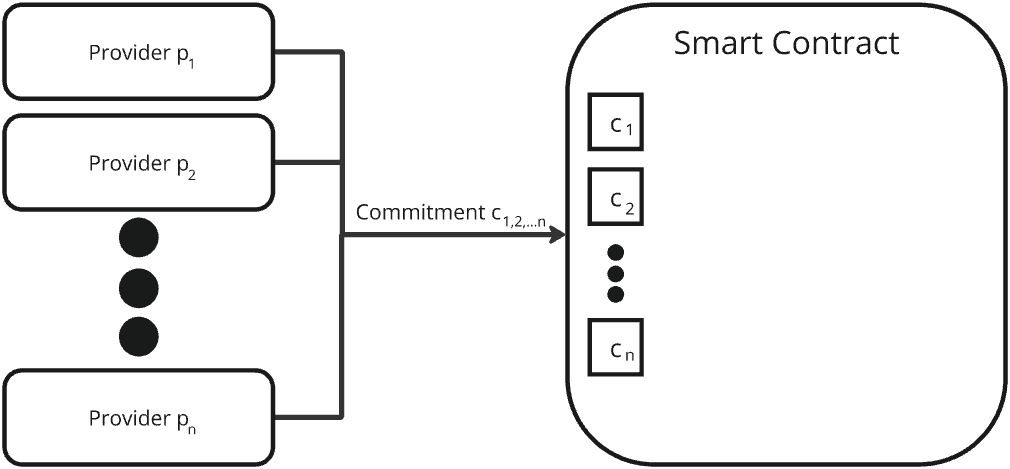
\includegraphics[width=0.8\textwidth]{images/commitment-stage.png}
\caption{Commitment Stage: Providers simultaneously submit hash commitments of their entropy values}
\label{fig:commitment-stage}
\end{figure}

\begin{figure}[h]
\centering
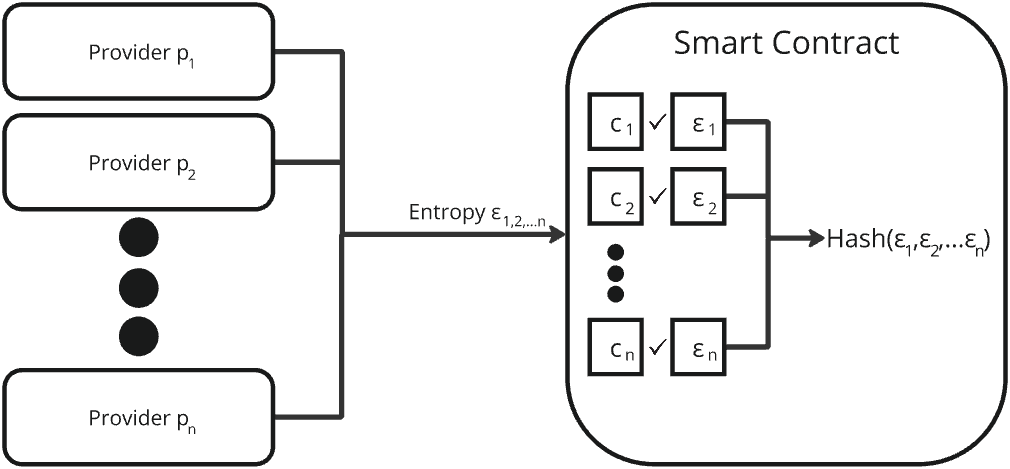
\includegraphics[width=0.8\textwidth]{images/reveal-stage.png}
\caption{Reveal Stage: Providers reveal their original entropy values which are verified against their commitments. After verification, a verifiable entropy unknown to any individual provider is created using a hash function}
\label{fig:reveal-stage}
\end{figure}

The protocol consists of the following key steps:

\begin{enumerate}
    \item \textbf{Provider Commitment}: Each provider $p_i$ commits to their entropy by submitting $c_i = \text{hash}(\varepsilon_i)$ to the smart contract
    \item \textbf{Provider Entropy}: After all commitments are received, providers reveal their original entropy values $\varepsilon_i$
    \item \textbf{Verification}: The smart contract verifies each revealed entropy matches its commitment by checking $c_i = \text{hash}(\varepsilon_i)$
    \item \textbf{Entropy Aggregation}: After all submitted entropies are verified, a verifiable entropy unknown to any of the individual providers is created using a method such as a hash function
\end{enumerate}

\subsubsection{Naive Implementation Vulnerability}\label{sec:commit_reveal_vulnerability}

While this naive commit-reveal scheme achieves decentralization, it suffers from a critical any-malicious denial of service vulnerability. Consider the following lottery scenario:

Suppose a lottery is being conducted with an insurmountable monetary reward. A single malicious provider can exploit the protocol through the following attack vector:

\begin{enumerate}
    \item The malicious provider initially follows the protocol through the commitment step, submitting their hash commitment like other participants.

    \item During the entropy revelation step, this provider (who may have purchased any number of lottery tickets) can wait until all other providers have revealed their entropy values.

    \item At this moment, the malicious actor can calculate the final outcome of the lottery by combining:
    \begin{itemize}
        \item All revealed entropy values from honest providers
        \item Their own private (yet unrevealed) entropy
    \end{itemize}

    \item With knowledge of the final outcome, the malicious actor can:
    \begin{itemize}
        \item If favorable: reveal their entropy and allow the lottery to complete
        \item If unfavorable: withhold their entropy, forcing a protocol restart and a new chance at a favorable outcome
    \end{itemize}
\end{enumerate}

This vulnerability demonstrates how a single malicious actor can repeatedly force redraws until achieving their desired outcome, effectively compromising the fairness of any high-stakes random number generation. Replacing the hash commitment with a time-lock puzzle closes it: the withheld value can always be recovered, so withholding no longer changes the outcome.

\subsection{Oracle Based VRF}\label{sec:oracle_based_vrf}
Chainlink's Verifiable Random Function (VRF)~\cite{chainlink_vrf} is based on the VRF construction proposed by Goldberg et al.~\cite{goldbergVRF}. The Goldberg VRF creates a pseudorandom number that is verifiable by the public. However, as noted in their work, it ``guarantees that $\beta$ is indistinguishable from random by anyone who does not know the secret key SK.'' Conversely, this implies that anyone in possession of the secret key can predict the ''random'' output.

This reliance on secret key holder(s) creates a fundamental trust assumption. Chainlink's implementation depends entirely on the trustworthiness of Chainlink and their ability to secure their secret key from hackers and corruption, creating a single point of failure.

\subsection{Threshold Signature Beacons}\label{sec:threshold_beacons}
A threshold beacon splits one signing key across $n$ parties so that any $t$ of them can sign a round number, and the unique BLS signature of that round becomes its random value. No single party can bias the output and missing parties do not stop it. The trust assumption, however, is $t$-of-$n$: any $t$ colluding parties can compute every future round in advance. RandAO offers such a beacon as its fast \texttt{quick} tier, for applications where that assumption is acceptable, and keeps the any-honest time-lock beacon for everything else.

\clearpage
\section{RandAO Protocol}\label{sec:protocol}

\subsection{Overview}\label{sec:protocol_overview}

The RandAO protocol builds upon the commit-reveal scheme discussed in Section~\ref{sec:related_work_commit_reveal}, replacing hash commitments with time-lock puzzles (Section~\ref{sec:timelock}). A set of validators $\mathcal{V} = \{v_1, \ldots, v_n\}$ produces a value per \emph{round}; every pending request is bound to a round and receives its own value derived from the round's output.

\begin{figure}[H]
\centering
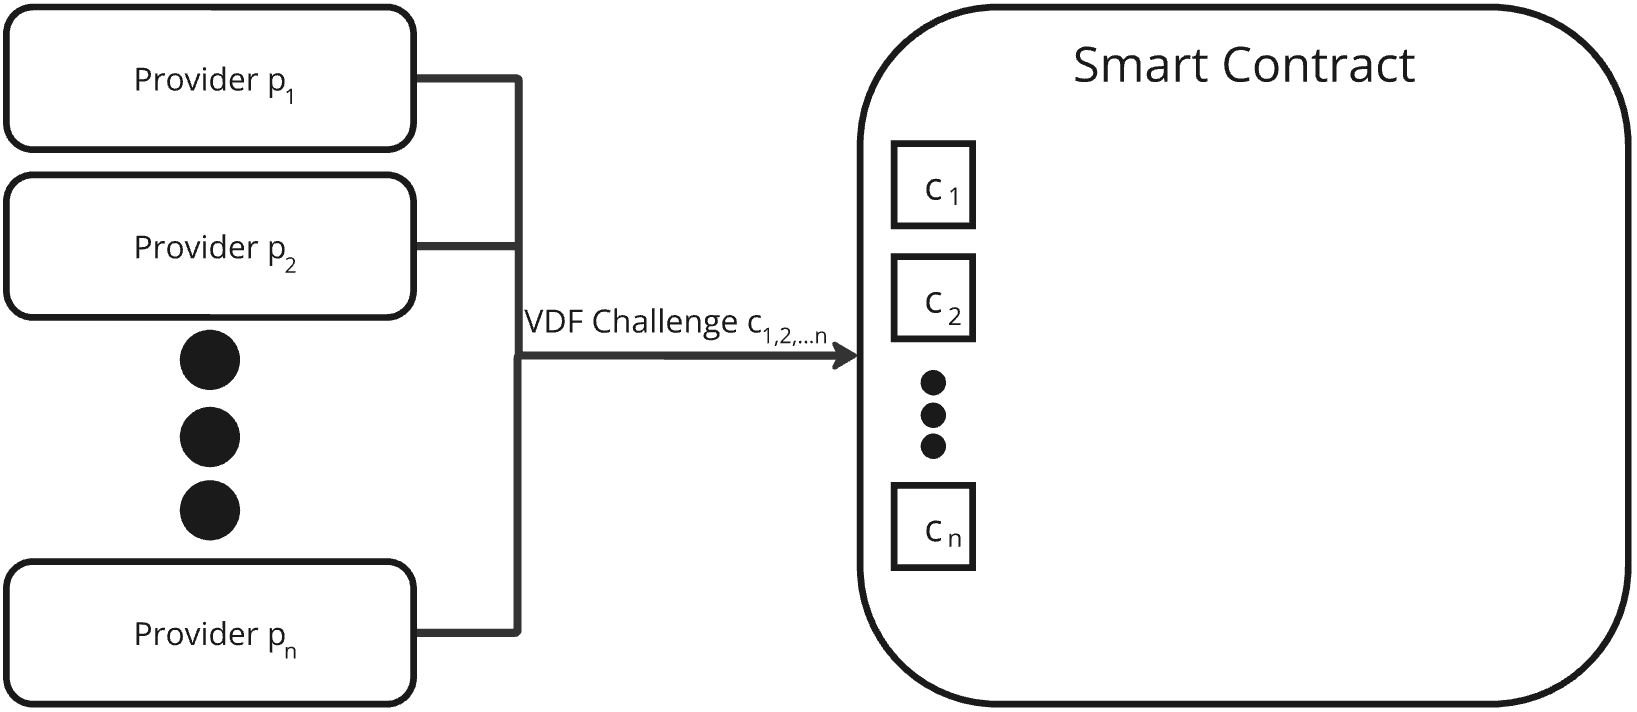
\includegraphics[width=0.8\textwidth]{images/protocol_commitment_phase.png}
\caption{Commitment: every validator posts its puzzle to the beacon process before the window closes}
\label{fig:protocol_commitment}
\end{figure}

\subsection{Puzzles}\label{sec:puzzles}

Each validator prepares RSA moduli ahead of time, $N = p \cdot q$ with $p$ and $q$ random primes of 1024 bits. Generating a 1024-bit prime takes about 18~ms on a commodity CPU, so a validator keeps a small pool. A modulus is used for exactly one round.

The puzzle input is not chosen by the validator; it is fixed by the round:
\begin{align*}
    \text{seed} &= \text{beacon} \,\|\, r \,\|\, v_i \\
    x &= \big(\text{expand}(\text{seed}) \bmod N\big)^2 \bmod N
\end{align*}
where $\text{expand}$ stretches the seed with SHA-256 to the size of $N$ plus 64 bits. The validator's contribution to round $r$ is
\begin{equation}
    y_i = x^{2^T} \bmod N ,
\end{equation}
which it computes instantly with its trapdoor (39~ms in Node.js at 2048 bits and $T = 2^{27}$) and which anyone else can compute only through $T$ sequential squarings.

\subsection{Round}\label{sec:round}

A round opens when requests are waiting. Requests bind to the open round until its first commitment; later requests wait for the next round.

\begin{enumerate}
    \item \textbf{Commit}: Each active validator posts its modulus $N_i$. The first commitment starts a commitment window of length $W$; commitments after the window are refused. Because $x$ is fixed by the round, posting $N_i$ fixes $y_i$.

    \item \textbf{Reveal}: Each committed validator posts $y_i$ together with one factor $p_i$ of $N_i$. The beacon checks the reveal through the \texttt{timelock@1.0} device: $1 < p_i < N_i$, $p_i \mid N_i$, and
    \begin{equation}
        y_i = x^{\,2^T \bmod (p_i-1)(q_i-1)} \bmod N_i .
    \end{equation}
    Publishing the factor is safe because the modulus is never used again.

    \item \textbf{Crack}: If a committed validator has not revealed by the reveal deadline, any validator may compute its $y_i$ by sequential squaring and post it with a Wesolowski proof (Section~\ref{sec:vdf}), which the device checks. The cracker earns the withholder's fee for the round, and the withholder receives a strike.

    \item \textbf{Aggregation}: When every committed $y_i$ is known, the round value is
    \begin{equation}
        V_r = \text{SHA-256}\big(\texttt{"rng/timelock"} \,\|\, \text{beacon} \,\|\, r \,\|\, y_{1} \,\|\, \cdots \,\|\, y_{k}\big)
    \end{equation}
    with the contributions ordered by validator address, and each request receives $\text{SHA-256}(V_r \,\|\, \text{requestId})$.
\end{enumerate}

If fewer than a minimum number of validators commit, the round is void and its requests move to the next round. The beacon stores every round's commitments, reveals, cracks and value, so anyone can re-verify any result.

\subsection{Any-Honest Security}\label{sec:any_honest}

Suppose validator $v_h$ is honest. When the commitment window closes, $y_h$ is fixed, but nobody except $v_h$ can compute it before $T$ sequential squarings, which by construction take longer than the window even on an attacker's fastest hardware. A dishonest validator deciding whether to commit therefore cannot know the round's value, and a dishonest validator deciding whether to reveal cannot change it, since its own $y_i$ is fixed and recoverable by cracking. The output is unpredictable and unbiasable unless every committed validator colludes.

\begin{figure}[H]
\centering
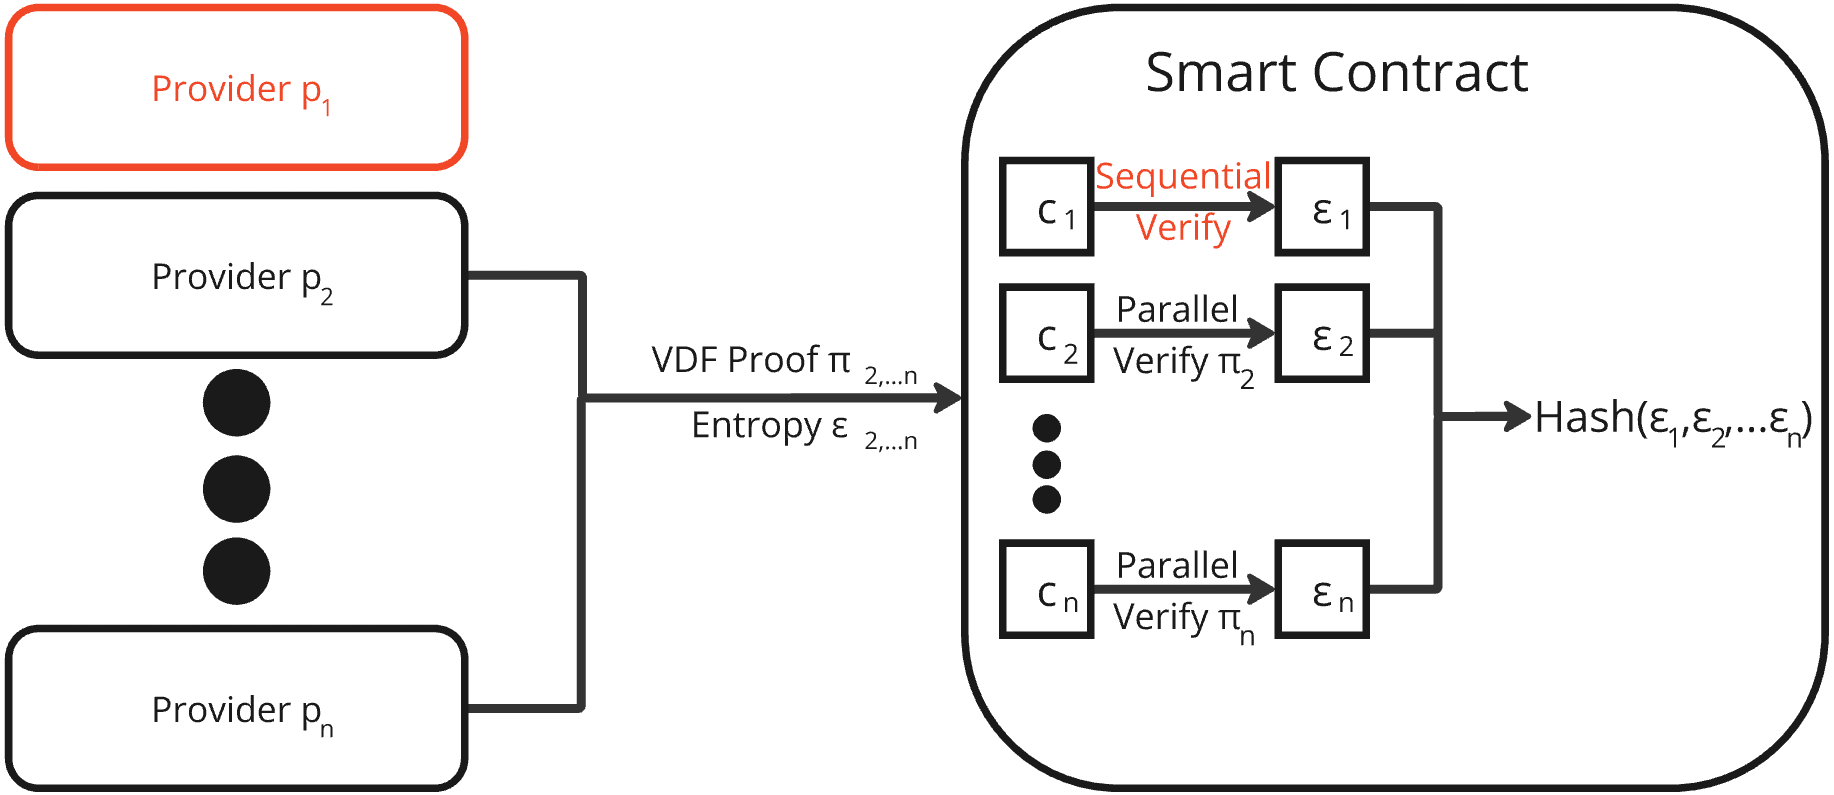
\includegraphics[width=0.8\textwidth]{images/verify-malicious-case.png}
\caption{A withholding validator cannot abort the round: its contribution is recovered by sequential computation from its commitment}
\label{fig:verify_malicious}
\end{figure}

\subsection{Timing}\label{sec:timing}

The parameters that set the protocol's timing are the number of squarings $T$, the commitment window $W$ and the reveal window $R$. Security requires
\begin{equation}
    \tau = \frac{T}{s_{\max}} > W ,
\end{equation}
where $s_{\max}$ is the squaring rate of the fastest hardware an attacker may own. The default $T = 2^{27}$ against an assumed $s_{\max}$ of $10^{7}$ squarings per second (ten times a fast CPU) gives $\tau \geq 13$~s against $W = 3$~s.

\subsubsection{Case: Standard}
Commitments arrive within the window, reveals follow immediately, and each reveal is checked with one exponentiation. A round costs two messages per validator and completes in a few seconds; requests that arrive while a round runs are batched into the next one.

\subsubsection{Case: A Validator Withholds}
The remaining validators wait until the reveal deadline and crack the missing puzzle. Native squaring runs at roughly one step per microsecond, so cracking and proving take a few minutes; JavaScript runs at about 14~$\mu$s per step and is only a fallback. The round is delayed, never changed.

\subsection{Validators}\label{sec:validators}

Validators are kept in a set by the beacon and are added or removed by the protocol's administrator, effective from the next round. Each validator signs its messages with its own wallet and generates its own puzzles; validators share no secret and need no key ceremony. A missed commitment or a cracked reveal is a strike; a validator with three strikes in a hundred rounds is suspended until reinstated, and a suspended validator neither commits nor earns. Opening the set to outside operators is planned once the protocol has run in production.

\subsection{Verification on the Node}\label{sec:device}

Our first version verified Pietrzak checkpoints by splitting each proof across a fleet of verifier processes, which cost dozens of messages per request. In the second version every check runs inside the node through the \texttt{timelock@1.0} HyperBEAM device. A reveal costs one modular exponentiation and a crack two short ones. The device is stateless and deterministic, so every node that computes or replays the beacon reaches the same verdict.

\clearpage
\section{Tiers}\label{sec:tiers}

\subsection{One Library}\label{sec:library}
Applications use RandAO through one Lua library. Every call names a continuation that receives a deterministic random stream, so moving a call site from one tier to another changes one option and nothing else:
\begin{verbatim}
rng.request(msg, { tier = "timelock", on = "Loot-Roll" })
\end{verbatim}
A stream offers integers without modulo bias, floats, picks and shuffles, and draws the same numbers on every node and every replay.

\subsection{The Tiers}\label{sec:tier_table}

\begin{center}
\begin{tabular}{p{2.2cm} p{4.2cm} p{3.6cm} p{1.8cm} p{1.4cm}}
\textbf{Tier} & \textbf{Source} & \textbf{Who can cheat} & \textbf{Latency} & \textbf{Price} \\
\hline
\texttt{local} & SHA-256 stream over the message & the sender, by re-signing & none & free \\
\texttt{quick} & threshold-BLS round, $t$ of $n$ validators & $t$ colluding validators & $\sim$1~s & $t+1$ RNG \\
\texttt{timelock} & time-lock commit-reveal of every validator & all validators together & a few seconds & $n+1$ RNG \\
\end{tabular}
\end{center}

The \texttt{local} tier needs no network and suits cosmetic effects and low-value draws. The \texttt{quick} tier answers in about a second and suits frequent game events. The \texttt{timelock} tier carries RandAO's any-honest guarantee and suits anything worth attacking: lotteries, rare drops, tournament brackets, validator selection.

\clearpage
\section{RNG Economy}\label{sec:rng_economics}

\subsection{Token Utility}\label{sec:token_utility}
The \$RNG token is the utility token of the RandAO ecosystem. Every paid randomness request is paid in \$RNG, which establishes a continuous demand that grows with the protocol's adoption.

\subsection{Prepaid Balances}\label{sec:balances}
Applications fund a balance in the beacon process by transferring \$RNG to it. Each request debits the balance when it is made, so no token transfer happens per request and a request costs a single message. A request with too little balance is refused with an error stating the balance and the price; it is never silently served at a weaker tier.

\subsection{Price Rule}\label{sec:price_rule}
The price of a request is one \$RNG for each validator whose contribution served it, plus one \$RNG for the protocol. With three validators, a \texttt{timelock} request costs four \$RNG and a \texttt{quick} request with a threshold of two costs three. Fees accrue inside the beacon and are claimed in batches. A validator that withholds a reveal forfeits its fee for that round to the validator that cracked it.

\subsection{Validators Without Staking}\label{sec:no_staking}
The first version required providers to stake collateral. Collateral only secures a protocol when it is worth more than an attack would gain, and requiring real value from every operator limited who could run a node. The second version starts without staking: the any-honest guarantee does not depend on collateral, and misbehaviour is answered with lost fees, strikes and suspension. Staking can return when the validator set opens to outside operators.

\clearpage
\section{Applications}\label{sec:applications}

\subsection{Gaming}\label{sec:applications_gaming}
Multiplayer video games extensively use random mechanics that directly impact player experiences and in-game economies. From critical hit calculations to loot drops and lootbox mechanics, players invest significant time and resources based on these probabilities. The fairness of these systems directly affects player satisfaction and game balance. With tiers in one library, a game can use free local randomness for cosmetic effects, the \texttt{quick} tier for frequent combat rolls and the \texttt{timelock} tier for rare drops and prizes.

This need for verifiable randomness extends naturally into gambling applications, where every slot machine pull, card shuffle, and dice roll must be demonstrably random and tamper-proof to maintain player trust. The stakes are often significant, making manipulation attempts a serious concern.

\subsection{NFTs}\label{sec:applications_nfts}
Non-Fungible Tokens (NFTs), such as those from the Bored Ape Yacht Club (BAYC)~\cite{boredapeyachtclub}, are typically generated by combining various image layers to create unique digital collectibles. Because of the Onchain Randomness Problem these are frequently created off-chain by developers and then uploaded, a process that can be manipulated. Verifiable onchain randomness enables provably fair and transparent minting.

\subsection{Proof of Stake Consensus}\label{sec:applications_defi}
Randomness is extensively utilized in Proof of Stake (PoS) consensus mechanisms. For instance, Solana employs random selection to determine the next leader in its consensus process~\cite{yakovenko2025solana}. This method ensures a fair and unpredictable rotation among validators.

\subsection{Artificial Intelligence}\label{sec:applications_security}
Random values are essential in neural networks such as large language models because they help the system learn. One of the most important uses of randomness is weight initialization, where the initial values of connections are set unpredictably so that different neurons learn different features~\cite{glorot2010understanding}.

\clearpage
\section{Future Developments}\label{sec:opportunities}

This section explores enhancements to the RandAO protocol that are not yet under development but would provide significant additional value.

\subsection{Time-Lock Encryption}\label{sec:timelock_encryption}
The puzzles that secure the beacon can also seal data. A message encrypted under a puzzle's answer stays sealed until the puzzle is solved, which enables sealed-bid auctions, hidden card hands, commit-reveal games without a reveal step and fair launches. The same device that verifies beacon reveals can verify that a sealed value was opened correctly.

\subsection{Open Validator Set}\label{sec:open_set}
The launch validators are run by RandAO Labs. Opening the set to outside operators, with admission rules and, where it adds security, staking, would make collusion progressively harder as the set grows: under the any-honest guarantee every additional independent validator is another party an attacker must corrupt.

\subsection{Subscription RNG Service Layer}\label{sec:subscription_service}
A subscription layer would let applications receive a stream of values per round rather than requesting each one, reducing messages further and enabling negotiated pricing such as volume discounts and fixed-rate packages.

\subsection{Honey Pot Mechanism}\label{sec:honey_pot}
A honey pot would reward anyone who proves a validator set is colluding by predicting a round's value before it is revealed. A correct prediction is evidence that validators leaked or coordinated their contributions; the reward would come from the colluding validators' fees, or their stake once staking exists. The mere existence of the mechanism deters collusion, since any member of a collusion could turn whistleblower.

\clearpage
\section{Outro}\label{sec:outro}

This whitepaper has outlined the ``\textbf{Onchain Randomness Problem}'' and why it now affects every AO process: HyperBEAM's runtime no longer offers \texttt{math.random}, because node-local randomness forks process state and can be steered by whoever controls the seed.

RandAO brings it back safely, as the first tool in a suite of cryptographic tools for the new age of the internet. One library gives every process deterministic randomness for free and upgrades the same call to verifiable randomness when value is at stake. Its flagship tier keeps the any-honest time-lock commit-reveal RandAO was founded on: as long as a single validator is honest, nobody can predict or bias a draw, and a validator who withholds can only delay it. Checking each reveal with the puzzle's one-time trapdoor inside the node, through the \texttt{timelock@1.0} device, makes that guarantee fast and cheap. Time-lock encryption follows on the same puzzles.

The \$RNG token pays for randomness: one token to each validator that served a request and one to the protocol. RandAO runs on testnet today, with launch validators operated by RandAO Labs; opening the validator set comes next.


\clearpage
\bibliographystyle{IEEEtran}
\bibliography{references}

\end{document}
